\documentclass{standalone}
\usepackage{graphicx}	
\usepackage{amssymb, amsmath, amsthm}
\usepackage{color}

\usepackage{tikz}
\usetikzlibrary{math, calc}

\definecolor{light}{RGB}{220, 188, 188}
\definecolor{mid}{RGB}{185, 124, 124}
\definecolor{dark}{RGB}{143, 39, 39}
\definecolor{highlight}{RGB}{180, 31, 180}
\definecolor{gray10}{gray}{0.1}
\definecolor{gray20}{gray}{0.2}
\definecolor{gray30}{gray}{0.3}
\definecolor{gray40}{gray}{0.4}
\definecolor{gray60}{gray}{0.6}
\definecolor{gray70}{gray}{0.7}
\definecolor{gray80}{gray}{0.8}
\definecolor{gray90}{gray}{0.9}
\definecolor{gray95}{gray}{0.95}
  
\newcommand{\drawcube}[4]{
  \pgfmathsetmacro{\dx}{#1}
  \pgfmathsetmacro{\dy}{#2} 
  \pgfmathsetmacro{\dz}{#3}  
  \pgfmathsetmacro{\tilt}{#4}
  
  \fill[light]    ({-(1 - \tilt) * \dx}, -\dy + \dz) 
               -- ({(1 + \tilt) * \dx}, -\dy + \dz) 
               -- ({(1 - \tilt) * \dx}, \dy + \dz) 
               -- ({-(1 + \tilt) * \dx}, \dy + \dz) -- cycle;  

  \fill[mid]    ({-(1 - \tilt) * \dx}, -\dy) 
             -- ({-(1 - \tilt) * \dx}, -\dy + \dz)
             -- ({-(1 + \tilt) * \dx}, \dy + \dz) 
						 -- ({-(1 + \tilt) * \dx}, \dy) -- cycle;

  \fill[dark]    ({-(1 - \tilt) * \dx}, -\dy) 
              -- ({(1 + \tilt) * \dx}, -\dy)
              -- ({(1 + \tilt) * \dx}, -\dy + \dz) 
              -- ({-(1 - \tilt) * \dx}, -\dy + \dz) -- cycle;
                       
  \draw[dark]    ({(1 + \tilt) * \dx}, -\dy) 
              -- ({(1 + \tilt) * \dx}, -\dy + \dz) 
              -- ({(1 - \tilt) * \dx}, \dy + \dz) 
              -- ({-(1 + \tilt) * \dx}, \dy + \dz)
              -- ({-(1 + \tilt) * \dx}, \dy) 
              -- ({-(1 - \tilt) * \dx}, -\dy)
              -- cycle;
              
 \draw[dark]    ({-(1 + \tilt) * \dx + 0.01}, \dy + \dz) 
             -- ({-(1 - \tilt) * \dx + 0.01}, -\dy + \dz) 
             -- ({(1 + \tilt) * \dx + 0.01}, -\dy + \dz);
}

\newcommand{\drawcubecageback}[4]{
  \pgfmathsetmacro{\dx}{#1}
  \pgfmathsetmacro{\dy}{#2} 
  \pgfmathsetmacro{\dz}{#3}  
  \pgfmathsetmacro{\tilt}{#4}
                   
  \draw[dark, dashed]    ({(1 - \tilt) * \dx}, \dy) 
                      -- ({(1 - \tilt) * \dx}, \dy + \dz) 
                      -- ({-(1 + \tilt) * \dx}, \dy + \dz) 
                      -- ({-(1 + \tilt) * \dx}, \dy) 
                      -- cycle;
}

\newcommand{\drawcubecagefront}[4]{
  \pgfmathsetmacro{\dx}{#1}
  \pgfmathsetmacro{\dy}{#2} 
  \pgfmathsetmacro{\dz}{#3}  
  \pgfmathsetmacro{\tilt}{#4}
                   
  \draw[dark, dashed]    ({(1 + \tilt) * \dx}, -\dy) 
                      -- ({(1 + \tilt) * \dx}, -\dy + \dz) 
                      -- ({-(1 - \tilt) * \dx + 0.015}, -\dy + \dz) 
                      -- ({-(1 - \tilt) * \dx + 0.015}, -\dy) 
                      -- cycle;
                      
  \draw[dark, dashed]    ({-(1 + \tilt) * \dx + 0.01}, \dy + \dz) 
                      -- ({-(1 - \tilt) * \dx + 0.01}, -\dy + \dz);

  \draw[dark, dashed]    ({(1 - \tilt) * \dx}, \dy + \dz) 
                      -- ({(1 + \tilt) * \dx}, -\dy + \dz);
             
}

\begin{document}

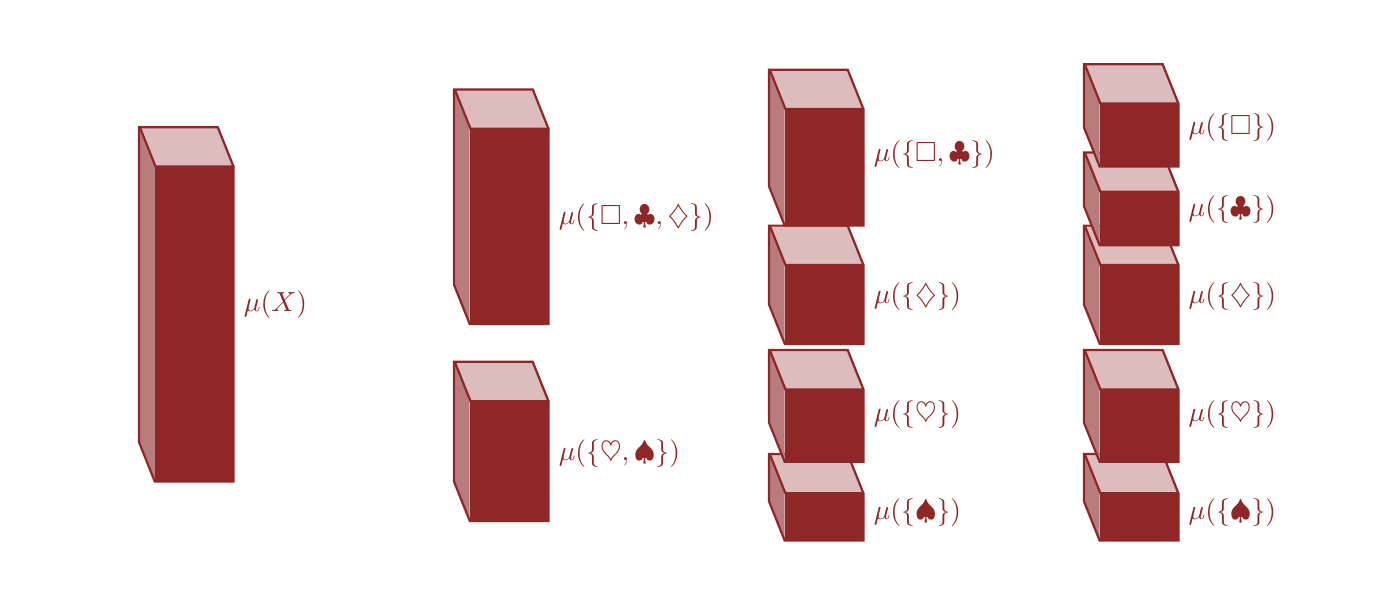
\begin{tikzpicture}[scale=1, thick]

  \draw[white] (-2, -3.5) rectangle (15, 3.5);
  
  \pgfmathsetmacro{\Dx}{4}
  
  \pgfmathsetmacro{\dx}{0.5}
  \pgfmathsetmacro{\dy}{0.25}
  \pgfmathsetmacro{\dz}{1}
  \pgfmathsetmacro{\tilt}{0.2}
  
  \begin{scope}[shift={(0, -2)}]
    \drawcube{\dx}{\dy}{4}{\tilt}
  \end{scope}

  \foreach \y/\p [count=\n] in {-2.5/0.38, -0/0.62} {
    \pgfmathsetmacro{\x}{\Dx}
    \begin{scope}[shift={(\x, \y)}]
      \drawcube{\dx}{\dy}{4 * \p}{\tilt}
    \end{scope}
  }

  \foreach \y\p [count=\n] in {-2.75/0.15, -1.75/0.23, -0.25/0.25, 1.25/0.37} {
    \pgfmathsetmacro{\x}{2 * \Dx}
    \begin{scope}[shift={(\x, \y)}]
      \drawcube{\dx}{\dy}{4 * \p}{\tilt}
    \end{scope}
  }

  \foreach \y/\p [count=\n] in {-2.75/0.15, -1.75/0.23, -0.25/0.25, 1/0.17, 2/0.2} {
    \pgfmathsetmacro{\x}{3 * \Dx}
    \begin{scope}[shift={(\x, \y)}]
      \drawcube{\dx}{\dy}{4 * \p}{\tilt}
    \end{scope}
  }
  
  \node[dark, anchor=west] at (0.6, 0) { $\mu(X)$ };
  
  \node[dark, anchor=west] at (\Dx + 0.6, 1.1) { $\mu( \{ \Box, \clubsuit, \diamondsuit \})$ };
  \node[dark, anchor=west] at (\Dx + 0.6, -1.9) { $\mu( \{ \heartsuit, \spadesuit \})$ };

  \node[dark, anchor=west] at (2 * \Dx + 0.6, 1.9) { $\mu( \{ \Box, \clubsuit \})$ };
  \node[dark, anchor=west] at (2 * \Dx + 0.6, 0.1) { $\mu( \{ \diamondsuit \})$ };
  \node[dark, anchor=west] at (2 * \Dx + 0.6, -1.4) { $\mu( \{ \heartsuit \})$ };
  \node[dark, anchor=west] at (2 * \Dx + 0.6, -2.65) { $\mu( \{ \spadesuit \})$ };

  \node[dark, anchor=west] at (3 * \Dx + 0.6, 2.25) { $\mu( \{ \Box \})$ };
  \node[dark, anchor=west] at (3 * \Dx + 0.6, 1.2) { $\mu( \{ \clubsuit \})$ };
  \node[dark, anchor=west] at (3 * \Dx + 0.6, 0.1) { $\mu( \{ \diamondsuit \})$ };
  \node[dark, anchor=west] at (3 * \Dx + 0.6, -1.4) { $\mu( \{ \heartsuit \})$ };
  \node[dark, anchor=west] at (3 * \Dx + 0.6, -2.65) { $\mu( \{ \spadesuit \})$ };

\end{tikzpicture}

\end{document}  